\documentclass[11pt, a4paper]{article}

% Pacchetti base per lingua e codifica
\usepackage[utf8]{inputenc}
\usepackage[italian]{babel}

% Pacchetti per la matematica e la fisica
\usepackage{amsmath, amssymb, amsfonts}
\usepackage{cancel} % Utile per sbarrare i termini che si annullano

% Pacchetti per la grafica e l'impaginazione
\usepackage{graphicx}
\usepackage{geometry}
\geometry{top=2.5cm, bottom=2.5cm, left=2.5cm, right=2.5cm}
\usepackage{booktabs}
\usepackage{multirow}
\usepackage{sectsty}
\usepackage{float}
\usepackage{xcolor}
\allsectionsfont{\underline}
\setcounter{secnumdepth}{0}

\begin{document}
\tableofcontents

\newpage

\section{Momento Angolare Intrinseco: Spin} %

Prima di introdurre lo Spin vero e proprio, studiamo il momento magnetico generato dal moto orbitale dell'elettrone. Partiamo dal \textbf{Principio di Equivalenza di Ampère}: %
Una spira percorsa da corrente $i$ che racchiude un'area $S$ si comporta come un dipolo magnetico infinitesimo: %
\begin{figure}[H]
    \centering
    \begin{minipage}{0.3\textwidth}
        \centering
        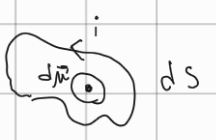
\includegraphics[width=\linewidth]{immagini/2026-05-07-14-59-28.png}
    \end{minipage}\hfill
    \begin{minipage}{0.65\textwidth}
        \begin{equation*}
            d\vec{\mu} = i \, dS \, \hat{u}_n %
        \end{equation*}
    \end{minipage}
\end{figure}

\noindent
Immerso in un campo magnetico $\vec{B}$, questo dipolo subisce un momento torcente $\vec{\tau}$ e possiede un'energia potenziale $U_{dip}$: %
\begin{figure}[H]
    \centering
    \begin{minipage}{0.3\textwidth}
        \centering
        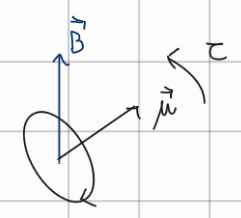
\includegraphics[width=\linewidth]{immagini/2026-05-07-14-59-48.png}
    \end{minipage}\hfill
    \begin{minipage}{0.65\textwidth}
        \begin{equation*}
            \vec{\tau} = \vec{\mu} \wedge \vec{B} \quad , \quad U_{dip} = -\vec{\mu} \cdot \vec{B} %
        \end{equation*}
    \end{minipage}
\end{figure}

\subsection{Fisica Atomica (Momento Magnetico Orbitale)} %

Consideriamo l'elettrone ($e^-$) che orbita attorno al nucleo ($e^+$) con velocità $v$ a distanza $r$. L'orbita costituisce una spira percorsa da una corrente media $i = \frac{e}{T}$, dove $T = \frac{2\pi r}{v}$ è il periodo di rivoluzione: %
\begin{figure}[H]
    \centering
    \begin{minipage}{0.3\textwidth}
        \centering
        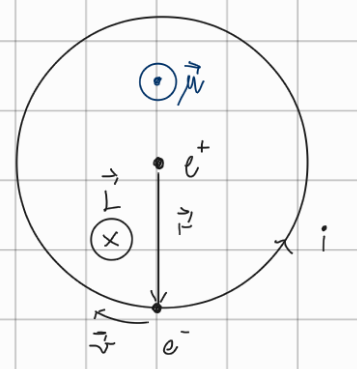
\includegraphics[width=\linewidth]{immagini/2026-05-07-15-00-39.png}
    \end{minipage}\hfill
    \begin{minipage}{0.65\textwidth}
        \begin{equation*}
            i = \frac{e}{\frac{2\pi r}{v}} = \frac{e v}{2\pi r} %
        \end{equation*}
        
        Il momento magnetico orbitale è quindi: %
        \begin{equation*}
            \vec{\mu} = i S \hat{u}_n = \frac{e v}{2\pi r} (\pi r^2) \hat{u}_n = \frac{e v r}{2} \hat{u}_n %
        \end{equation*}
    \end{minipage}
\end{figure}

\noindent
Moltiplichiamo e dividiamo per la massa $m$ dell'elettrone per far emergere il momento angolare $\vec{L} = \vec{r} \wedge (m\vec{v})$: %
\begin{equation*}
    \vec{\mu} = \frac{e}{2m} (m v r) \hat{u}_n = -\frac{e}{2m} \vec{L} %
\end{equation*}
\textit{(Nota: Il segno meno indica che, essendo l'elettrone carico negativamente, il momento magnetico $\vec{\mu}$ è antiparallelo al momento angolare $\vec{L}$).} %

\noindent
Nella fisica delle particelle, la proporzionalità tra momento angolare e momento magnetico è una legge generale. Il coefficiente di proporzionalità $\gamma$ prende il nome di \textbf{Rapporto Giromagnetico}: %
\begin{equation}
    \boxed{ \vec{\mu} = \gamma \vec{L} \quad \Rightarrow \quad \gamma = -\frac{e}{2m} } %
\end{equation}

\subsection{Precessione di Larmor e Diamagnetismo} %

Cosa succede se poniamo questo "atomo" in un campo magnetico uniforme $\vec{B}$? L'equazione del moto per il momento angolare è dettata dal momento torcente: %
\begin{equation*}
    \frac{d\vec{L}}{dt} = \vec{\tau} \text{ (MOM. TORCENTE)} = \vec{\mu} \wedge \vec{B} = \left(-\frac{e}{2m}\vec{L}\right) \wedge \vec{B} = \frac{e}{2m} \vec{B} \wedge \vec{L} %
\end{equation*}

\begin{figure}[H]
    \centering
    \begin{minipage}{0.3\textwidth}
        \centering
        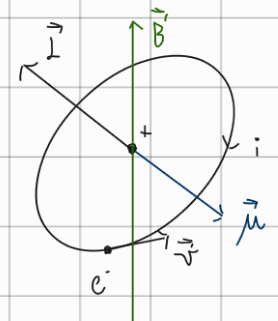
\includegraphics[width=0.7\linewidth]{immagini/2026-05-07-15-02-40.png}
    \end{minipage}\hfill
    \begin{minipage}{0.65\textwidth}
        Dalla cinematica rotazionale sappiamo che se la derivata di un vettore è data dal prodotto vettoriale con una velocità angolare ($\frac{d\vec{L}}{dt} = \vec{\omega} \wedge \vec{L}$), allora il vettore compie un moto di precessione. 
        Confrontando le equazioni, otteniamo la \textbf{Frequenza di Precessione di Larmor ($\vec{\omega}_L$)}: %
        \begin{equation}
            \frac{d\vec{L}}{dt} = \vec{\omega}_L \wedge \vec{L} \quad \Rightarrow \quad \vec{\omega}_L = \frac{e}{2m}\vec{B} %
        \end{equation}
    \end{minipage}
\end{figure}

Da questa equazione differenziale derivano tre conseguenze fondamentali: %
\begin{enumerate}
    \item $a.\quad |\vec{L}| = \text{COST}$ (Il modulo si conserva) %
    \item $b.\quad \frac{d}{dt}(\vec{L}\cdot\vec{B}) = 0 \Rightarrow \angle(\vec{L}, \vec{B})$ RESTA COSTANTE (L'angolo non cambia) %
    \item $c.\quad$ Il vettore $\vec{L}$ (e conseguentemente $\vec{\mu}$) \textbf{RUOTA ATTORNO A $\vec{B}$} con velocità angolare $|\vec{\omega}_L| = \frac{e|\vec{B}|}{2m}$. %
\end{enumerate}

\begin{figure}[H]
    \centering
    \begin{minipage}{0.3\textwidth}
        \centering
        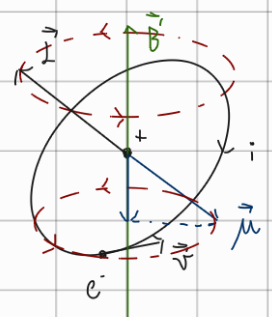
\includegraphics[width=0.7\linewidth]{immagini/2026-05-07-15-02-57.png}
    \end{minipage}\hfill
    \begin{minipage}{0.65\textwidth}
        \textit{Questo fenomeno microscopico è l'origine fisica del \textbf{Diamagnetismo}. Tuttavia, la velocità di precessione (per $B \simeq 1\text{ T}$) è $\omega_L \simeq 10^{11} \text{ rad/s}$, che è gigantesca a livello macroscopico ma trascurabile rispetto alla frequenza orbitale di Bohr dell'elettrone ($\omega_0 \simeq 10^{16} \text{ rad/s}$).} %
    \end{minipage}
\end{figure}

\subsection{Campo Magnetico Non Uniforme (Forza di Deflessione)} %

Se il campo magnetico \textbf{NON} è uniforme, oltre al momento torcente nasce una vera e propria forza di traslazione spaziale, data dal gradiente dell'energia potenziale: %
\begin{equation*}
    \vec{F} = -\nabla U_{dip} = -\nabla(-\vec{\mu} \cdot \vec{B}) = \nabla(\vec{\mu} \cdot \vec{B}) %
\end{equation*}
Se il campo varia solo lungo l'asse $z$ (cioè $\vec{B} = B_z(z)\hat{u}_z$), la forza deflettente è proporzionale alla componente $z$ del momento magnetico: %
\begin{equation}
    \vec{F} = \mu_z \frac{\partial B_z}{\partial z} \hat{u}_z %
\end{equation}

\subsection{Quantizzazione e Magnetone di Bohr} %

Passando alla meccanica quantistica, sappiamo che l'unità naturale per il momento angolare è $\hbar$. Riscriviamo $\vec{\mu}$ esplicitando $\hbar$: %
\begin{equation*}
    \vec{\mu} = -\frac{e}{2m}\vec{L} = -\frac{e\hbar}{2m} \frac{\vec{L}}{\hbar} = -g_l \mu_B \frac{\vec{L}}{\hbar} %
\end{equation*}

Abbiamo introdotto due quantità fondamentali: %
\begin{enumerate}
    \item Il \textbf{Fattore g-orbitale ($g_l$)}: Per il momento angolare orbitale, esso vale esattamente $1$ ($g_l = 1$). %
    \item Il \textbf{Magnetone di Bohr ($\mu_B$)}: Il "quanto" fondamentale di momento magnetico atomico: %
    \begin{equation}
        \boxed{ \mu_B = \frac{e\hbar}{2m} \simeq 9.3 \cdot 10^{-24} \text{ J/T} = 5.8 \cdot 10^{-5} \text{ eV/T} } %
    \end{equation}
\end{enumerate}

\noindent
Essendo il momento angolare $\vec{L}$ quantizzato, lo è anche il momento magnetico orbitale $\vec{\mu}$! Sostituendo gli autovalori noti di $\hat{L}^2$ e $\hat{L}_z$: %
\begin{align}
    |\vec{L}| &= \hbar \sqrt{l(l+1)} \quad \Rightarrow \quad \boxed{ |\vec{\mu}| = \mu_B \sqrt{l(l+1)} } \\ %
    L_z &= \hbar m \quad \Rightarrow \quad \mu_z = -g_l \mu_B \frac{L_z}{\hbar} \quad \Rightarrow \quad \boxed{ \mu_z = -\mu_B m } %
\end{align}

\noindent
\textbf{Conclusione Spettacolare:} %
Sostituiamo $\mu_z$ nell'equazione della forza subita dall'atomo nel campo magnetico non uniforme: %
\begin{equation}
    \vec{F} = \left(-\mu_B m \right) \frac{\partial B_z}{\partial z} \hat{u}_z %
\end{equation}
La forza di deflessione $\vec{F}$ è una \textbf{funzione diretta del numero quantico magnetico $m$}. Poiché $m$ può assumere solo valori interi discreti ($-l \dots +l$), un fascio di atomi inviato in un gradiente di campo magnetico si separerà in un \textbf{numero discreto e quantizzato di tracce}! %

\section{L'Esperimento di Stern-Gerlach (1923)} %

\begin{figure}[H]
    \centering
    \begin{minipage}{0.3\textwidth}
        \centering
        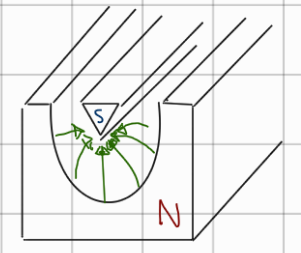
\includegraphics[width=\linewidth]{immagini/2026-05-07-15-05-43.png}
    \end{minipage}\hfill
    \begin{minipage}{0.65\textwidth}
        Per verificare la quantizzazione spaziale del momento angolare, Stern e Gerlach idearono un esperimento fondamentale. Un fascio di atomi vaporizzati da un forno viene fatto passare attraverso un magnete con un campo magnetico fortemente non uniforme ($\frac{\partial B_z}{\partial z} \simeq 1000 \text{ T/m}$, molto più forte verso la "punta" del magnete). %
    \end{minipage}
\end{figure}

Sappiamo che la forza deflettente sul fascio è $\vec{F}_z = \mu_z \frac{\partial B_z}{\partial z} \hat{u}_z$. Vediamo le previsioni teoriche rispetto al risultato sullo schermo: %

\begin{enumerate}
    \item \textbf{Fisica Classica:} Il momento magnetico $\mu_z$ può assumere valori continui. Ci si aspetta una \textbf{striscia continua} (macchia allungata) sullo schermo. %
    \item \textbf{Meccanica Quantistica (Previsione):} Sappiamo che $L_z$ è quantizzato, con $(2l+1)$ valori. 
    \begin{itemize}
        \item Se lo stato avesse $l=2$, ci aspetteremmo $5$ macchie distinte ($m = -2, -1, 0, 1, 2$). %
        \item L'esperimento fu condotto con atomi di Argento ($Ag$). L'Argento ha un solo elettrone di valenza nel guscio $5s$, quindi \textbf{il suo momento angolare orbitale è nullo ($l=0$)}. Di conseguenza, $\mu_z = 0$. %
        \item \textbf{Ipotesi Teorica:} Essendo $l=0 \Rightarrow m=0$, il fascio non dovrebbe subire alcuna deflessione. Ci si aspetta \textbf{1 sola macchia centrale}! %
    \end{itemize}
    \begin{figure}[H]
        \centering
        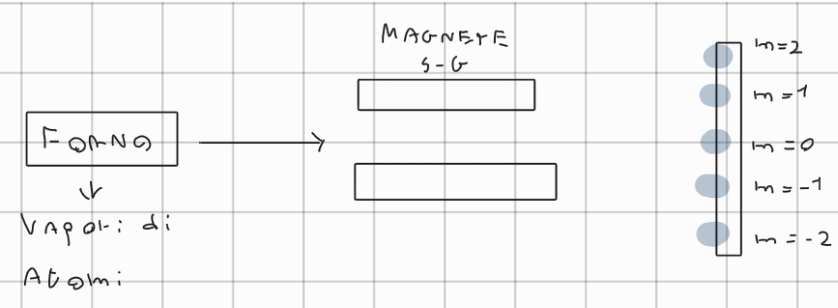
\includegraphics[width=0.6\linewidth]{immagini/2026-05-07-15-07-14.png}
        \end{figure}
    \item \textbf{REALTÀ SPERIMENTALE:} Il fascio si divide in \textbf{2 macchie distinte} (una deviata in alto, una in basso)! %
    \begin{figure}[H]
        \centering
        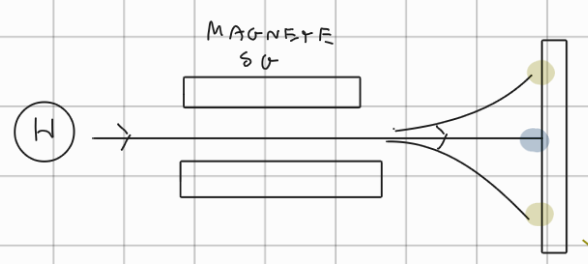
\includegraphics[width=0.5\linewidth]{immagini/2026-05-07-15-07-37.png}
        \end{figure}
\end{enumerate}

\subsection{Il Mistero delle Due Macchie} %

Perché l'atomo di Argento viene deflesso in due tracce se il suo momento angolare orbitale è zero? Escludiamo alcune ipotesi: %
\begin{itemize}
    \item \textit{Magari $l \neq 0$?} Falso. Qualsiasi valore di $l$ intero produce un numero dispari di macchie ($2l+1$), mai un numero pari come 2! %
    \item \textit{Magari è dovuto alle cariche nel nucleo?} Il nucleo ha un suo momento magnetico, ma essendo proporzionale alla massa del protone, il magnetone nucleare è $\mu_B^N = \frac{e\hbar}{2m_p}$. È circa $10^{-3}$ volte più piccolo del magnetone di Bohr dell'elettrone, la forza sarebbe impercettibile. Falso! %
\end{itemize}
\textit{Nota sperimentale:} L'esperimento non si può fare sparando elettroni liberi, perché la forza di deflessione sarebbe sovrastata dalla Forza di Lorentz ($\vec{F}_L = q\vec{v}\wedge\vec{B}$). Usando atomi neutri di Ag, l'unica forza netta è quella sul dipolo. %

\noindent
\textbf{LA SOLUZIONE (1925):} La forza $\vec{F}_z = \mu_z \frac{\partial B_z}{\partial z}$ deve provenire da un momento magnetico di dipolo associato a un \textbf{Momento Angolare Intrinseco} dell'elettrone stesso. Questo grado di libertà venne chiamato \textbf{SPIN}. %

\begin{figure}[H]
    \centering
    \begin{minipage}{0.2\textwidth}
        \centering
        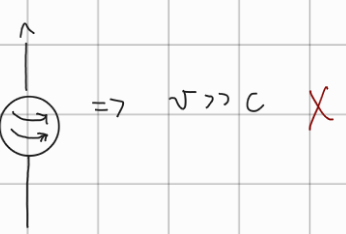
\includegraphics[width=\linewidth]{immagini/2026-05-07-15-11-00.png}
    \end{minipage}\hfill
    \begin{minipage}{0.75\textwidth}
        \textbf{Cos'è lo Spin?} All'inizio si pensava all'elettrone che "ruota su sé stesso" come una trottola. Ma calcolando la velocità periferica necessaria per generare quel momento magnetico per una particella così piccola, si otterrebbe una velocità della superficie $v \gg c$ (maggiore della luce), il che viola la relatività. %
        $\Rightarrow$ \textbf{Lo Spin è un grado di libertà puramente quantistico che NON ha alcun analogo classico.} %
    \end{minipage}
\end{figure}

\subsection{Formalismo dell'Operatore di Spin $\hat{S}$} %

Dai risultati dell'esperimento (conoscendo il gradiente del campo $\frac{\partial B_z}{\partial z}$ e misurando la deflessione spaziale delle due macchie), Stern e Gerlach poterono calcolare il valore esatto di $\mu_z$: %
\begin{equation}
    \boxed{ \mu_z = \pm \mu_B } \quad \Rightarrow \text{Mom. di dipolo magnetico intrinseco quantizzato per } e^- %
\end{equation}

Per analogia con il momento orbitale $\vec{L}$, introduciamo il momento angolare di Spin $\vec{S}$: %
\begin{align*}
    \vec{\mu}_l = -g_l \mu_B \frac{\vec{L}}{\hbar} \quad &\Rightarrow \quad \vec{\mu}_s = -g_s \mu_B \frac{\vec{S}}{\hbar} \\ %
    (\mu_l)_z = -g_l \mu_B m_l \quad &\Rightarrow \quad (\mu_s)_z = -g_s \mu_B m_s %
\end{align*}
Dove $g_s$ è il fattore giromagnetico di spin e $m_s$ il numero quantico magnetico di spin. %

\noindent
\textbf{Teoria del Momento Angolare Generale ($\vec{J}$):} %
Si può dimostrare matematicamente che, basandosi unicamente sulle regole di commutazione, per un \textbf{QUALUNQUE} operatore di momento angolare $\vec{J}$ valgono le seguenti proprietà (legate al corpo di simmetrie spaziali rotazionali): %
\begin{equation}
    [\hat{J}^2, \hat{J}_i] = 0 \qquad \text{e} \qquad [\hat{J}_i, \hat{J}_j] = \varepsilon_{ijk} i\hbar \hat{J}_k %
\end{equation}
Da queste si deduce che gli autovalori di $J^2$ sono $\hbar^2 j(j+1)$, dove il numero quantico $j$ può assumere non solo valori interi, ma anche \textbf{seminteri}: %
\begin{align*}
    j &= 0, \frac{1}{2}, 1, \frac{3}{2}, 2, \dots \\ %
    m_j &= -j, -j+1, \dots, +j \quad (\text{Totale di } 2j+1 \text{ stati}) %
\end{align*}
L'operatore orbitale $\hat{L}$ studiato finora è solo un \textit{sottoinsieme} dei momenti $\vec{J}$ generali (quello ristretto ai soli valori interi). %

\subsection{Deduzione del Valore dello Spin ($s=1/2$)} %

Applichiamo l'algebra generale $\vec{J}$ all'operatore di Spin $\hat{S}$. Le sue regole di commutazione sono identiche: %
\begin{equation*}
    [\hat{S}^2, \hat{S}_z] = 0 \quad , \quad [\hat{S}_x, \hat{S}_y] = i\hbar \hat{S}_z \dots %
\end{equation*}
Con gli autovalori: %
\begin{equation}
    S^2 = \hbar^2 s(s+1) \qquad \text{e} \qquad S_z = \hbar m_s \qquad \text{con } m_s = -s, \dots, +s %
\end{equation}

\noindent
Sappiamo sperimentalmente che l'esperimento genera \textbf{esattamente DUE macchie} simmetriche. Questo significa che la proiezione $m_s$ può assumere solo $2$ valori. %
Poiché $m_s$ salta sempre di un'unità discreta ($+1$), gli unici due valori simmetrici possibili distanti $1$ tra loro sono: %
\begin{equation*}
    m_s = -\frac{1}{2} \quad \text{e} \quad m_s = +\frac{1}{2} \quad \Rightarrow \quad s = \frac{1}{2} %
\end{equation*}
\textbf{Il numero quantico di SPIN per l'elettrone è SEMINTERO!} %

\noindent
Inoltre, sapendo che l'esperimento fissa la magnetizzazione a $(\mu_s)_z = \pm \mu_B$, uguagliandola alla nostra formula teorica: %
\begin{equation}
    (\mu_s)_z = \pm \mu_B = -g_s \mu_B m_s = -g_s \mu_B \left(\pm \frac{1}{2}\right) \quad \Rightarrow \quad \boxed{ g_s = 2 } %
\end{equation}
A differenza del momento orbitale ($g_l = 1$), il fattore giromagnetico di spin per l'elettrone vale $2$ (l'elettrone è due volte più "efficace" nel generare momento magnetico col suo spin rispetto alla sua orbita). %

\subsection{Conclusione e Relatività (Dirac, 1928)} %

Il problema concettuale rimane: \textbf{L'Equazione di Schrödinger NON PREVEDE lo Spin.} È stato aggiunto artificialmente (postulato) per far tornare i conti con l'esperimento di Stern-Gerlach. %

\noindent
Il trionfo teorico arrivò solo pochi anni dopo, nel 1928, ad opera di \textbf{Paul Dirac}. %
Unendo la Meccanica Quantistica alla \textbf{Teoria della Relatività Ristretta} ($E = \sqrt{p^2 c^2 + m^2 c^4} + V$), Dirac formulò la celebre "Equazione di Dirac". 
Risolvendo questa equazione relativistica, l'esistenza dello Spin e l'esatto valore di $g_s=2$ emergono \textbf{naturalmente} e inevitabilmente dalla struttura matematica dello spazio-tempo! %

\begin{quote}
    \textbf{LO SPIN $\Leftrightarrow$ È UN EFFETTO DELLA RELATIVITÀ.} %
\end{quote}

\section{Lo Spin delle Particelle} %

Lo spin è una proprietà intrinseca fondamentale della materia. Particelle diverse possiedono numeri quantici di spin ($S$) differenti: %
\begin{itemize}
    \item Elettroni, Protoni, Neutroni $\Rightarrow S = 1/2$ (Fermioni) %
    \item Mesoni $\pi$ (quark + antiquark) $\Rightarrow S = 0$ (Bosoni) %
    \item Fotoni $\Rightarrow S = 1$ (Bosoni) %
    \item Barioni $\Delta$ (3 quark) $\Rightarrow S = 3/2$ %
\end{itemize}

\noindent
\begin{figure}[H]
    \centering
    \begin{minipage}{0.3\textwidth}
        \centering
        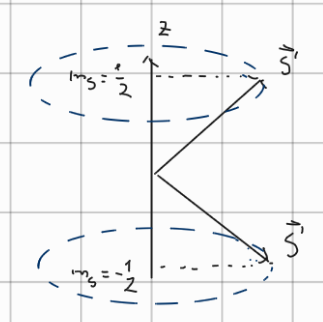
\includegraphics[width=\linewidth]{immagini/2026-05-07-15-16-17.png}
    \end{minipage}\hfill
    \begin{minipage}{0.65\textwidth}
        Concentriamoci sugli \textbf{Elettroni}. Avendo $S = 1/2$, il numero quantico magnetico di spin può assumere solo due valori: $m_s = \pm 1/2$. %
        Di conseguenza, la proiezione del momento angolare di spin lungo l'asse $z$ è limitata a due stati discreti: %
        \begin{equation*}
            S_z = \pm \frac{\hbar}{2} %
        \end{equation*}
    \end{minipage}
\end{figure}

\noindent
Poiché il sistema ha esattamente due stati possibili, lo \textbf{Spazio di Hilbert} associato allo spin non è più uno spazio funzionale a infinite dimensioni, ma un semplice \textbf{Spazio Vettoriale 2D}. %
Possiamo descriverlo usando due versori di base ortonormali: $\vec{u}_1 = \begin{pmatrix} 1 \\ 0 \end{pmatrix}$ e $\vec{u}_2 = \begin{pmatrix} 0 \\ 1 \end{pmatrix}$. %

\noindent
Uno stato generico sarà una combinazione lineare: $\vec{u} = \alpha \vec{u}_1 + \beta \vec{u}_2$, con la condizione di normalizzazione $|\alpha|^2 + |\beta|^2 = 1$. %

\noindent
Utilizzando la notazione di Dirac (Bra-Ket), lo stato colonna (Ket) e il suo duale riga complesso coniugato (Bra) si scrivono come: %
\begin{equation*}
    |\psi\rangle = \begin{pmatrix} \psi_1 \\ \psi_2 \end{pmatrix} \qquad , \qquad \langle\psi| = \begin{pmatrix} \psi_1^* & \psi_2^* \end{pmatrix} %
\end{equation*}

In questo spazio 2D, \textbf{GLI OPERATORI SONO MATRICI} $2\times 2$: %
\begin{equation*}
    \hat{O} \Rightarrow \hat{O} = \begin{bmatrix} O_{11} & O_{12} \\ O_{21} & O_{22} \end{bmatrix} \qquad \text{con l'operatore aggiunto } \hat{O}^\dagger = (\hat{O}^T)^* %
\end{equation*}

Le regole di commutazione generali rimangono valide per queste matrici: %
\begin{equation*}
    [\hat{S}^2, \hat{S}_i] = 0 \qquad \text{e} \qquad [\hat{S}_i, \hat{S}_j] = i\hbar\varepsilon_{ijk}\hat{S}_k %
\end{equation*}

\subsection{Spinori (La Funzione d'Onda di Spin)} %

Lo stato quantistico del sistema (la parte di spin della funzione d'onda) prende il nome di \textbf{SPINORE}. %
Essendo $[\hat{S}^2, \hat{S}_z] = 0$, essi condividono una base di autovettori comuni. Definiamo gli autovettori di $\hat{S}_z$: %

\begin{itemize}
    \item \textbf{SPIN-UP:} Indicato con $|\uparrow\rangle$ o $\chi_+$. Corrisponde a $S_z = +\hbar/2$. %
    \begin{equation*}
        \chi_+ = |\uparrow\rangle = \begin{pmatrix} 1 \\ 0 \end{pmatrix} %
    \end{equation*}
    \item \textbf{SPIN-DOWN:} Indicato con $|\downarrow\rangle$ o $\chi_-$. Corrisponde a $S_z = -\hbar/2$. %
    \begin{equation*}
        \chi_- = |\downarrow\rangle = \begin{pmatrix} 0 \\ 1 \end{pmatrix} %
    \end{equation*}
\end{itemize}

Lo \textbf{Spinore Generico} è una combinazione di questi due stati fondamentali: %
\begin{equation}
    |\chi\rangle = a |\uparrow\rangle + b |\downarrow\rangle = \begin{pmatrix} a \\ b \end{pmatrix} \qquad \text{con } |a|^2 + |b|^2 = 1 %
\end{equation}
E il suo Bra corrispondente è $\langle\chi| = \begin{pmatrix} a^* & b^* \end{pmatrix}$. %

\noindent
Come per la funzione d'onda spaziale $\psi = \sum c_n \phi_n$, i coefficienti al quadrato rappresentano le probabilità di misura: %
\begin{itemize}
    \item $|a|^2 = \mathbb{P}\left(S_z = +\frac{\hbar}{2}\right)$ %
    \item $|b|^2 = \mathbb{P}\left(S_z = -\frac{\hbar}{2}\right)$ %
\end{itemize}

\noindent
Vogliamo trovare la forma esplicita delle matrici $2\times 2$ che rappresentano gli operatori $\hat{S}_z$ e $\hat{S}^2$. %
Sappiamo che l'equazione agli autovalori è $\hat{S}_z = \hbar m_s = \pm \frac{\hbar}{2}$. Applicando l'operatore matriciale incognito ai due vettori di base, dobbiamo ottenere il vettore stesso moltiplicato per l'autovalore: %

\begin{align*}
    \hat{S}_z |\uparrow\rangle &= S_z \begin{pmatrix} 1 \\ 0 \end{pmatrix} = +\frac{\hbar}{2} \begin{pmatrix} 1 \\ 0 \end{pmatrix} = +\frac{\hbar}{2} |\uparrow\rangle \\ %
    \hat{S}_z |\downarrow\rangle &= S_z \begin{pmatrix} 0 \\ 1 \end{pmatrix} = -\frac{\hbar}{2} \begin{pmatrix} 0 \\ 1 \end{pmatrix} = -\frac{\hbar}{2} |\downarrow\rangle %
\end{align*}

\noindent
L'unica matrice $2\times 2$ che soddisfa contemporaneamente queste due equazioni è una \textbf{matrice diagonale}: %
\begin{equation}
    \boxed{ \hat{S}_z = \frac{\hbar}{2} \begin{bmatrix} 1 & 0 \\ 0 & -1 \end{bmatrix} } %
\end{equation}

\noindent
Procediamo analogamente per l'operatore modulo quadro $\hat{S}^2$. Sappiamo che l'autovalore per $s=1/2$ è unico e vale $S^2 = \hbar^2 s(s+1) = \frac{3}{4}\hbar^2$. %
\begin{align*}
    \hat{S}^2 |\uparrow\rangle &= \hat{S}^2 \begin{pmatrix} 1 \\ 0 \end{pmatrix} = \frac{3}{4}\hbar^2 \begin{pmatrix} 1 \\ 0 \end{pmatrix} \\ %
    \hat{S}^2 |\downarrow\rangle &= \hat{S}^2 \begin{pmatrix} 0 \\ 1 \end{pmatrix} = \frac{3}{4}\hbar^2 \begin{pmatrix} 0 \\ 1 \end{pmatrix} %
\end{align*}
Anche in questo caso, la matrice è diagonale (ovviamente, dato che commuta con $\hat{S}_z$): %
\begin{equation}
    \boxed{ \hat{S}^2 = \frac{3}{4}\hbar^2 \begin{bmatrix} 1 & 0 \\ 0 & 1 \end{bmatrix} } %
\end{equation}
    
\noindent 
Per ricavare le altre due componenti spaziali ($\hat{S}_x$ e $\hat{S}_y$), si sfruttano le regole di commutazione (o gli operatori di salita e discesa). Le matrici risultanti sono \textbf{NON DIAGONALI} (poiché non commutano con $\hat{S}_z$): %
\begin{equation}
    \hat{S}_x = \frac{\hbar}{2} \begin{bmatrix} 0 & 1 \\ 1 & 0 \end{bmatrix} \qquad , \qquad \hat{S}_y = \frac{\hbar}{2} \begin{bmatrix} 0 & -i \\ i & 0 \end{bmatrix} %
\end{equation}

\subsection{Matrici di Pauli} %

Raccogliendo il fattore $\hbar/2$ dagli operatori di spin appena ricavati, definiamo le \textbf{Matrici di Pauli} ($\hat{\sigma}_x, \hat{\sigma}_y, \hat{\sigma}_z$): %

\begin{align*}
    \hat{\sigma}_x &= \begin{bmatrix} 0 & 1 \\ 1 & 0 \end{bmatrix} \quad \Rightarrow \quad \hat{S}_x = \frac{\hbar}{2} \hat{\sigma}_x \\ %
    \hat{\sigma}_y &= \begin{bmatrix} 0 & -i \\ i & 0 \end{bmatrix} \quad \Rightarrow \quad \hat{S}_y = \frac{\hbar}{2} \hat{\sigma}_y \\ %
    \hat{\sigma}_z &= \begin{bmatrix} 1 & 0 \\ 0 & -1 \end{bmatrix} \quad \Rightarrow \quad \hat{S}_z = \frac{\hbar}{2} \hat{\sigma}_z %
\end{align*}

\noindent
\textit{(Queste matrici sono intimamente legate al modo di ruotare dei vettori nell'Algebra di Lie)}. %
Proprietà matematiche fondamentali: le matrici di Pauli sono \textbf{HERMITIANE} ($\hat{\sigma}^\dagger = \hat{\sigma}$) e \textbf{UNITARIE} ($\hat{\sigma}_j^\dagger \hat{\sigma}_j = \mathbb{I}$). %

\subsection{Ricerca degli Autostati per le altre componenti} %

Ci chiediamo: lo stato di Spin-Up $|\uparrow\rangle = \binom{1}{0}$ (che è autostato di $\hat{S}_z$) è per caso anche autostato di $\hat{S}_x$? Verifichiamolo applicando l'operatore: %
\begin{equation*}
    \hat{S}_x |\uparrow\rangle = \frac{\hbar}{2} \begin{bmatrix} 0 & 1 \\ 1 & 0 \end{bmatrix} \binom{1}{0} = \frac{\hbar}{2} \binom{0}{1} = \frac{\hbar}{2} |\downarrow\rangle %
\end{equation*}
Poiché il risultato non è un multiplo dello stato di partenza, deduciamo che \textbf{NON È UN AUTOSTATO di $\hat{S}_x$} (non ridà sé stesso). %

\noindent
Calcoliamo quindi i veri autovalori e autovettori di $\hat{S}_x$. Impostiamo l'equazione caratteristica per il determinante: %
\begin{equation*}
    \det(\hat{S}_x - \lambda \mathbb{I}) = \begin{vmatrix} -\lambda & \hbar/2 \\ \hbar/2 & -\lambda \end{vmatrix} = 0 \quad \Rightarrow \quad \lambda^2 - \left(\frac{\hbar}{2}\right)^2 = 0 \quad \Rightarrow \quad \boxed{ \lambda = \pm \frac{\hbar}{2} } %
\end{equation*}
\textit{(Sorpresa: gli autovalori misurabili per l'asse x sono identici a quelli dell'asse z, come deve essere per l'isotropia dello spazio!)} %

Troviamo gli \textbf{Autovettori} associati sostituendo i $\lambda$: %
\begin{itemize}
    \item Per $\lambda = +\hbar/2$: %
    \begin{equation*}
        \begin{bmatrix} -\hbar/2 & \hbar/2 \\ \hbar/2 & -\hbar/2 \end{bmatrix} \binom{a}{b} = \binom{0}{0} \quad \Rightarrow \quad -\frac{\hbar}{2}a + \frac{\hbar}{2}b = 0 \quad \Rightarrow \quad a = b \quad \Rightarrow \quad |\chi_x^+\rangle = \begin{pmatrix} 1/\sqrt{2} \\ 1/\sqrt{2} \end{pmatrix} %
    \end{equation*}
    
    \item Per $\lambda = -\hbar/2$: %
    \begin{equation*}
        \begin{bmatrix} \hbar/2 & \hbar/2 \\ \hbar/2 & \hbar/2 \end{bmatrix} \binom{a}{b} = \binom{0}{0} \quad \Rightarrow \quad \frac{\hbar}{2}a + \frac{\hbar}{2}b = 0 \quad \Rightarrow \quad a = -b \quad \Rightarrow \quad |\chi_x^-\rangle = \begin{pmatrix} 1/\sqrt{2} \\ -1/\sqrt{2} \end{pmatrix} %
    \end{equation*}
\end{itemize}
Conclusione: Avendo autostati diversi, i due operatori non commutano: $\boxed{ [\hat{S}_z, \hat{S}_x] \neq 0 }$. %

\subsection{Misura delle Componenti dello Spin} %

Dato uno spinore generico $|\chi\rangle = \binom{a}{b}$, calcoliamo il \textbf{valore atteso} (valor medio) di una misura lungo z: %
\begin{align*}
    \langle \hat{S}_z \rangle &= \langle \chi | \hat{S}_z | \chi \rangle = \begin{pmatrix} a^* & b^* \end{pmatrix} \frac{\hbar}{2} \begin{bmatrix} 1 & 0 \\ 0 & -1 \end{bmatrix} \binom{a}{b} = \\ %
    &= \frac{\hbar}{2} (|a|^2 - |b|^2) = |a|^2 \left(+\frac{\hbar}{2}\right) + |b|^2 \left(-\frac{\hbar}{2}\right) %
\end{align*}
Questo coincide perfettamente con la definizione statistica $\langle A \rangle = \sum \mathbb{P}_n A_n$. %

\noindent
Se prepariamo il sistema nello stato puro $|\uparrow\rangle = \binom{1}{0}$, avremo: %
\begin{equation*}
    \langle \hat{S}_z \rangle = (1)\left(\frac{\hbar}{2}\right) + (0)\left(-\frac{\hbar}{2}\right) = \frac{\hbar}{2} \quad \text{(come al solito ho il 100\% di probabilità di misurare Up)} %
\end{equation*}

Ma cosa succede se cerchiamo di misurare $\hat{S}_x$ mentre il sistema si trova nello stato $|\uparrow\rangle$? %
\begin{equation*}
    \langle \hat{S}_x \rangle = \langle \uparrow | \hat{S}_x | \uparrow \rangle = \begin{pmatrix} 1 & 0 \end{pmatrix} \frac{\hbar}{2} \begin{bmatrix} 0 & 1 \\ 1 & 0 \end{bmatrix} \binom{1}{0} = 0 \quad \Rightarrow \quad \boxed{ \langle \hat{S}_x \rangle = 0 } %
\end{equation*}
Perché fa zero? Possiamo espandere lo stato $|\uparrow\rangle = \binom{1}{0}$ come \textbf{sovrapposizione degli autostati di $\hat{S}_x$}: %
\begin{equation*}
    \binom{1}{0} = \frac{1}{\sqrt{2}} \begin{pmatrix} 1/\sqrt{2} \\ 1/\sqrt{2} \end{pmatrix} + \frac{1}{\sqrt{2}} \begin{pmatrix} 1/\sqrt{2} \\ -1/\sqrt{2} \end{pmatrix} \quad \Rightarrow \quad |\uparrow\rangle_z = \frac{1}{\sqrt{2}} |\chi_x^+\rangle + \frac{1}{\sqrt{2}} |\chi_x^-\rangle %
\end{equation*}
I quadrati dei coefficienti sono $(\frac{1}{\sqrt{2}})^2 = \frac{1}{2}$. Se siamo in un autostato di $\hat{S}_z$, abbiamo esattamente il \textbf{50\%} di probabilità di misurare Spin-Up lungo X e il \textbf{50\%} di misurare Spin-Down lungo X! %
\begin{quote}
    \textit{Se sono in un autostato di $\hat{S}_z$, non posso conoscere con precisione $S_x$ e $S_y$!} %
\end{quote}

\begin{figure}[H]
    \centering
    \begin{minipage}{0.36\textwidth}
        \centering
        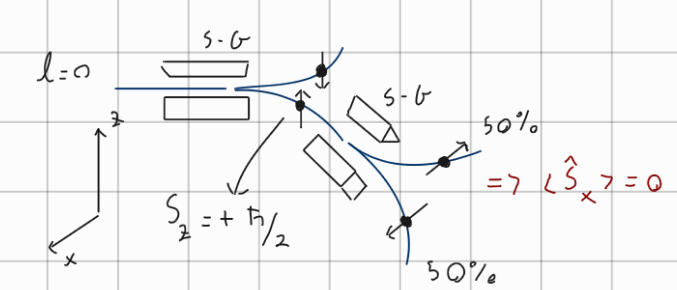
\includegraphics[width=\linewidth]{immagini/2026-05-07-15-26-29.png}
    \end{minipage}\hfill
    \begin{minipage}{0.63\textwidth}
        \textbf{L'Esperimento dei 3 Stern-Gerlach:} %
        Se sparo un fascio in un SG lungo $z$ e filtro solo la macchia superiore ($|\uparrow\rangle_z$), poi passo questo fascio puro in un SG orientato lungo l'asse $x$, il fascio si spaccherà di nuovo a metà (50\% su e 50\% giù rispetto a x). %
        \textit{Il paradosso:} Se prendo una delle due macchie uscenti dall'asse $x$ (es. $|\chi_x^+\rangle$) e la rimetto in un terzo SG \textbf{orientato di nuovo lungo z}, cosa ottengo? Non riottengo il 100\% di $|\uparrow\rangle_z$ iniziale! La misurazione lungo X ha "distrutto" la memoria del sistema, facendo \textbf{collassare la funzione d'onda}. Troverò di nuovo il 50\% di $\hat{S}_z$ Up e il 50\% Down! %
    \end{minipage}
\end{figure}

\subsection{La Funzione d'Onda Completa (Spazio + Spin)} %

Riscriviamo l'operatore di spin totale vettoriale per comodità: $\hat{\vec{S}} = \frac{\hbar}{2}\hat{\vec{\sigma}} = \frac{\hbar}{2}(\hat{\sigma}_x, \hat{\sigma}_y, \hat{\sigma}_z)$. %

\noindent
Fino ad ora abbiamo studiato l'atomo di Idrogeno con le sole coordinate spaziali $\vec{r}$. La parte spaziale era $u_{nlm}(\vec{r})$, riassumibile come $u_q(\vec{r}) \in \mathcal{L}^2(\mathbb{R}^3)$ con i quanti $q = \{n, l, m\}$. %
Dall'altra parte abbiamo lo Spinore $|\chi\rangle = \binom{a}{b}$ nello spazio di Hilbert 2D, con $a, b \in \mathbb{C}$ e $|a|^2+|b|^2 = 1$. %

\noindent
Mettiamo insieme i due spazi! La \textbf{Funzione d'Onda Completa} è un vettore a due componenti dipendente dalle coordinate: %
\begin{equation}
    \boxed{ u(\vec{r}, S_z) = \begin{pmatrix} a \, u_{q_1}(\vec{r}) \\ b \, u_{q_2}(\vec{r}) \end{pmatrix} } %
\end{equation}

\noindent
La condizione di normalizzazione complessiva (integro sullo spazio e sommo sullo spin) deve fare $1$: %
\begin{equation*}
    \int_{\mathbb{R}^3} |a \, u_{q_1}(\vec{r})|^2 \, d\vec{r} + \int_{\mathbb{R}^3} |b \, u_{q_2}(\vec{r})|^2 \, d\vec{r} = 1 %
\end{equation*}

\subsection{Esempi Pratici di Funzioni d'Onda Totali} %

a) \textbf{Stato puro spaziale e puro di spin:} %
\begin{equation*}
    u(\vec{r}, S_z) = u_{100} \binom{1}{0} \quad \Rightarrow \quad \text{L'elettrone si trova nel } \textbf{1s} \text{ ed è sicuramente } \textbf{Spin-UP} \text{ (100\% $\uparrow$)}. %
\end{equation*}

b) \textbf{Stato puro spaziale, misto di spin:} %
\begin{equation*}
    u(\vec{r}, S_z) = u_{100} \left[ \frac{1}{\sqrt{2}} \binom{1}{0} + \frac{1}{\sqrt{2}} \binom{0}{1} \right] \quad \Rightarrow \quad \text{Elettrone in } \textbf{1s} \text{, con 50\% di } \uparrow \text{ e 50\% di } \downarrow. %
\end{equation*}

c) \textbf{Stato combinato (Entangled Spazio-Spin):} %
\begin{equation*}
    u(\vec{r}, S_z) = \frac{1}{\sqrt{2}} u_{100} \binom{1}{0} + \frac{1}{\sqrt{2}} u_{200} \binom{0}{1} %
\end{equation*}
In questo caso, il sistema è in una sovrapposizione complessa: ho il 50\% di probabilità di trovare l'elettrone nello stato $\mathbf{1s}$ \textbf{e} con Spin $\mathbf{\uparrow}$, e il 50\% di probabilità di trovarlo nello stato $\mathbf{2s}$ \textbf{e} con Spin $\mathbf{\downarrow}$. %

\section{Somma di Momenti Angolari} %

Riassumiamo i momenti angolari noti. Le loro equazioni agli autovalori hanno tutte la medesima struttura matematica: %
\begin{align*}
    \text{Orbitale } \vec{L} &\Rightarrow L^2 = \hbar^2 l(l+1) \quad , \quad L_z = \hbar m_l \quad (m_l = -l \dots l) \\ %
    \text{Spin } \vec{S} &\Rightarrow S^2 = \hbar^2 s(s+1) \quad , \quad S_z = \hbar m_s \quad (m_s = \pm 1/2) \\ %
    \text{Generico } \vec{J} &\Rightarrow J^2 = \hbar^2 j(j+1) \quad , \quad J_z = \hbar m_j \quad (m_j = -j \dots j) %
\end{align*}
Ricordiamo i commutatori generali per $\vec{J}$: $[\hat{J}^2, \hat{J}_i] = 0$ e $[\hat{J}_i, \hat{J}_j] = i\hbar\varepsilon_{ijk}\hat{J}_k$. %

\noindent
Se un sistema possiede due momenti angolari $\vec{J}_1$ e $\vec{J}_2$, il momento angolare totale è la somma vettoriale $\vec{J} = \vec{J}_1 + \vec{J}_2$. %
Tuttavia, classicamente, per fare una somma vettoriale esatta dovrei conoscere simultaneamente tutte le componenti $(x, y, z)$. In meccanica quantistica questo è \textbf{impossibile} a causa del Principio di Indeterminazione. %
Possiamo però sommare con precisione le proiezioni lungo l'asse $z$ (i numeri quantici magnetici): %
\begin{equation*}
    m_j = m_{j_1} + m_{j_2} %
\end{equation*}

\subsection{Teorema di Somma dei Momenti Angolari} %

I valori permessi per il numero quantico totale $j$ non sono infiniti, ma seguono la regola della disuguaglianza triangolare (saltando di un'unità discreta): %
\begin{equation}
    \boxed{ j = |j_1 - j_2| , \, |j_1 - j_2| + 1 , \dots , j_1 + j_2 } \quad \text{SALTANDO DI } 1 %
\end{equation}

\noindent
\textbf{Esempio:} Siano $j_1 = 1$ e $j_2 = 3$. I valori possibili per il modulo totale $j$ sono: %
\begin{equation*}
    j = |1 - 3| \dots (1 + 3) \quad \Rightarrow \quad \textbf{j = 2, 3, 4} %
\end{equation*}
Ciascuno di questi stati di $j$ totale ha i suoi sottostati $m_j$: %
\begin{itemize}
    \item $j=4 \Rightarrow m_j = -4, \dots, 4$ %
    \item $j=3 \Rightarrow m_j = -3, \dots, 3$ %
    \item $j=2 \Rightarrow m_j = -2, \dots, 2$ %
\end{itemize}
Il valore massimo possibile della proiezione è coerentemente $\text{MAX} = j_1 + j_2 = j_{\text{max}}$. %

\begin{figure}[H]
    \centering
    \begin{minipage}{0.4\textwidth}
        \centering
        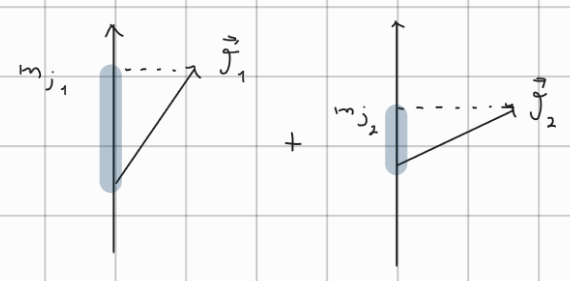
\includegraphics[width=\linewidth]{immagini/2026-05-07-15-33-05.png}
    \end{minipage}\hfill
    \begin{minipage}{0.1\textwidth}
        $\rightarrow$
    \end{minipage}
    \begin{minipage}{0.4\textwidth}
        \begin{figure}[H]
            \centering
            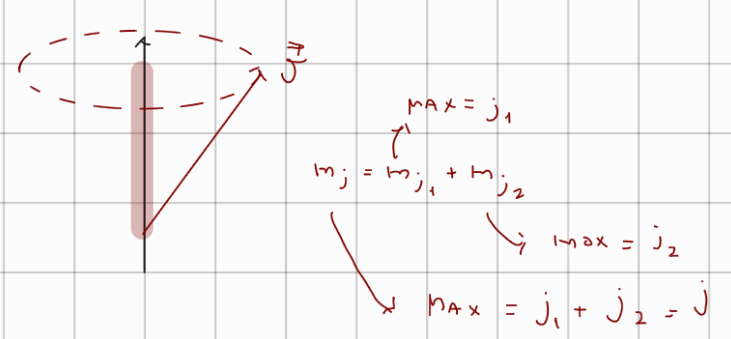
\includegraphics[width=\linewidth]{immagini/2026-05-07-15-32-52.png}
            \end{figure}
    \end{minipage}
\end{figure}

\subsection{La Base Disaccoppiata} %

Essendo $\vec{J}_1$ e $\vec{J}_2$ relativi a gradi di libertà o particelle diverse (es. orbitale e spin), essi sono \textbf{COMPLETAMENTE INDIPENDENTI}. Questo significa che qualsiasi componente di $\vec{J}_1$ commuta con qualsiasi componente di $\vec{J}_2$: %
\begin{equation*}
    [\hat{J}_1^2, \hat{J}_2^2] = 0 \quad , \quad [\hat{J}_1^2, \hat{J}_{2_i}] = 0 \quad , \quad [\hat{J}_{1_i}, \hat{J}_{2_k}] = 0 %
\end{equation*}

\noindent
Possiamo quindi trovare un set di \textbf{4 operatori che commutano mutuamente} e che condividono una base di autovettori in comune: %
\begin{equation*}
    \hat{J}_1^2 \quad , \quad \hat{J}_{1z} \quad , \quad \hat{J}_2^2 \quad , \quad \hat{J}_{2z} %
\end{equation*}
La base di autostati simultanei formata da questi operatori è chiamata \textbf{BASE DISACCOPPIATA}. Utilizzando la notazione di Dirac per indicare lo stato tramite i numeri quantici: %
\begin{equation}
    \boxed{ |j_1, m_{j_1}, j_2, m_{j_2}\rangle } %
\end{equation}

L'azione degli operatori è banale (ognuno "vede" solo il proprio pezzo): %
\begin{align*}
    \hat{J}_1^2 |j_1, m_{j_1}, j_2, m_{j_2}\rangle &= \hbar^2 j_1(j_1+1) |j_1, m_{j_1}, j_2, m_{j_2}\rangle \\ %
    \hat{J}_{1z} |j_1, m_{j_1}, j_2, m_{j_2}\rangle &= \hbar m_{j_1} |j_1, m_{j_1}, j_2, m_{j_2}\rangle \\
    \hat{J}_2^2 |j_1, m_{j_1}, j_2, m_{j_2}\rangle &= \hbar^2 j_2(j_2+1) |j_1, m_{j_1}, j_2, m_{j_2}\rangle \\ %
    \hat{J}_{2z} |j_1, m_{j_1}, j_2, m_{j_2}\rangle &= \hbar m_{j_2} |j_1, m_{j_1}, j_2, m_{j_2}\rangle
\end{align*}

\noindent
\textit{(Nota esplicativa formale: Usare i ket è come scrivere $\hat{H}|nlm\rangle = E_n|nlm\rangle$ per abbreviare $\hat{H}u_{nlm} = E_n u_{nlm}$).} %

\subsection{La Base Accoppiata e Clebsch-Gordan} %

Definiamo l'operatore quadrato del momento totale $\hat{J}^2$: %
\begin{equation*}
    \hat{J}^2 = (\hat{\vec{J}}_1 + \hat{\vec{J}}_2)^2 = \hat{J}_1^2 + \hat{J}_2^2 + 2\hat{\vec{J}}_1 \cdot \hat{\vec{J}}_2 = \hat{J}_1^2 + \hat{J}_2^2 + 2(\hat{J}_{1x}\hat{J}_{2x} + \hat{J}_{1y}\hat{J}_{2y} + \hat{J}_{1z}\hat{J}_{2z}) %
\end{equation*}

\noindent
Se calcoliamo i commutatori, scopriamo che $\hat{J}^2$ commuta con $\hat{J}_1^2$, $\hat{J}_2^2$ e $\hat{J}_z$. %
\textbf{ATTENZIONE:} $\hat{J}^2$ \textbf{NON} commuta con $\hat{J}_{1z}$ e $\hat{J}_{2z}$ (a causa dei termini crociati $x$ e $y$ nel prodotto scalare)! %
\begin{equation*}
    [\hat{J}^2, \hat{J}_{1z}] \neq 0 \quad , \quad [\hat{J}^2, \hat{J}_{2z}] \neq 0 %
\end{equation*}

\noindent
Dobbiamo quindi scegliere un \textbf{NUOVO SET di 4 operatori mutuamente commutanti}: %
\begin{equation*}
    \hat{J}^2 \quad , \quad \hat{J}_z \quad , \quad \hat{J}_1^2 \quad , \quad \hat{J}_2^2 %
\end{equation*}
Questo set definisce una nuova base, chiamata \textbf{BASE ACCOPPIATA}, che identifica rigorosamente il modulo del momento totale e la sua proiezione: %
\begin{equation}
    \boxed{ |j, m_j, j_1, j_2\rangle } %
\end{equation}

Con i seguenti autovalori sulle funzioni di base: %
\begin{align*}
    \hat{J}^2 |j, m_j, j_1, j_2\rangle &= \hbar^2 j(j+1) |j, m_j, j_1, j_2\rangle \\ %
    \hat{J}_z |j, m_j, j_1, j_2\rangle &= \hbar m_j |j, m_j, j_1, j_2\rangle \\ %
    \hat{J}_1^2 |j, m_j, j_1, j_2\rangle &= \hbar^2 j_1(j_1+1) |j, m_j, j_1, j_2\rangle \\ %
    \hat{J}_2^2 |j, m_j, j_1, j_2\rangle &= \hbar^2 j_2(j_2+1) |j, m_j, j_1, j_2\rangle %
\end{align*}

\noindent
Se i vettori formano basi complete per lo stesso spazio vettoriale, posso passare da una base all'altra tramite una trasformazione lineare (una matrice di rotazione). I coefficienti di questa combinazione lineare sono i \textbf{Coefficienti di Clebsch-Gordan} ($C_{m_{j_1}, m_{j_2}}^j$): %
\begin{equation}
    |j, m_j, j_1, j_2\rangle = \sum_{m_{j_1}, m_{j_2}} C_{m_{j_1}, m_{j_2}}^j |j_1, m_{j_1}, j_2, m_{j_2}\rangle %
\end{equation}

\section{Spin di Due Elettroni (Singoletto e Tripletto)} %

Cosa succede se abbiamo un sistema con due elettroni (es. atomo di Elio)? Dobbiamo sommare i loro spin intrinseci: %
\begin{equation*}
    s_1 = \frac{1}{2} \quad , \quad s_2 = \frac{1}{2} %
\end{equation*}

Applicando il Teorema di Somma dei momenti angolari per trovare lo Spin Totale $S$: %
\begin{equation*}
    S = |s_1 - s_2|, \dots , s_1 + s_2 \quad \Rightarrow \quad S = 0, \, 1 %
\end{equation*}

Il sistema a due elettroni può quindi trovarsi in due configurazioni di spin totale distinte: %
\begin{enumerate}
    \item \textbf{Se $\mathbf{S = 0}$:} La proiezione può essere solo $m_s = 0$. C'è un solo stato possibile, chiamato \textbf{SINGOLETTO}. I due vettori spin sono perfettamente opposti (antiparalleli, $\uparrow\downarrow$ o $\downarrow\uparrow$), annullandosi a vicenda. %
    \begin{figure}[H]
        \centering
        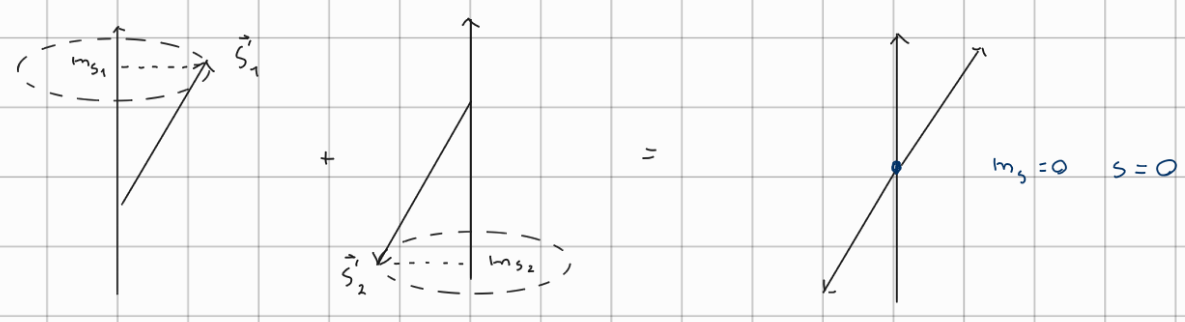
\includegraphics[width=0.8\linewidth]{immagini/2026-05-07-15-48-01.png}
        \end{figure}
    \item \textbf{Se $\mathbf{S = 1}$:} La proiezione può assumere $2S+1 = 3$ valori: $m_s = -1, 0, 1$. Questo macro-stato è chiamato \textbf{TRIPLETTO}. %
\end{enumerate}

\noindent
Le proiezioni si sommano in modo algebrico normale: $m_s = m_{s_1} + m_{s_2}$. %
Avendo $m_{s_1} = \pm 1/2$ e $m_{s_2} = \pm 1/2$, le combinazioni generano: %
\begin{align*}
    1/2 + 1/2 &= 1 \quad \Rightarrow \quad \uparrow\uparrow \quad (m_s = 1) \\ %
    1/2 - 1/2 &= 0 \quad \Rightarrow \quad \uparrow\downarrow \quad (m_s = 0) \\ %
    -1/2 + 1/2 &= 0 \quad \Rightarrow \quad \downarrow\uparrow \quad (m_s = 0) \\ %
    -1/2 - 1/2 &= -1 \quad \Rightarrow \quad \downarrow\downarrow \quad (m_s = -1) %
\end{align*}

\begin{figure}[H]
    \centering
    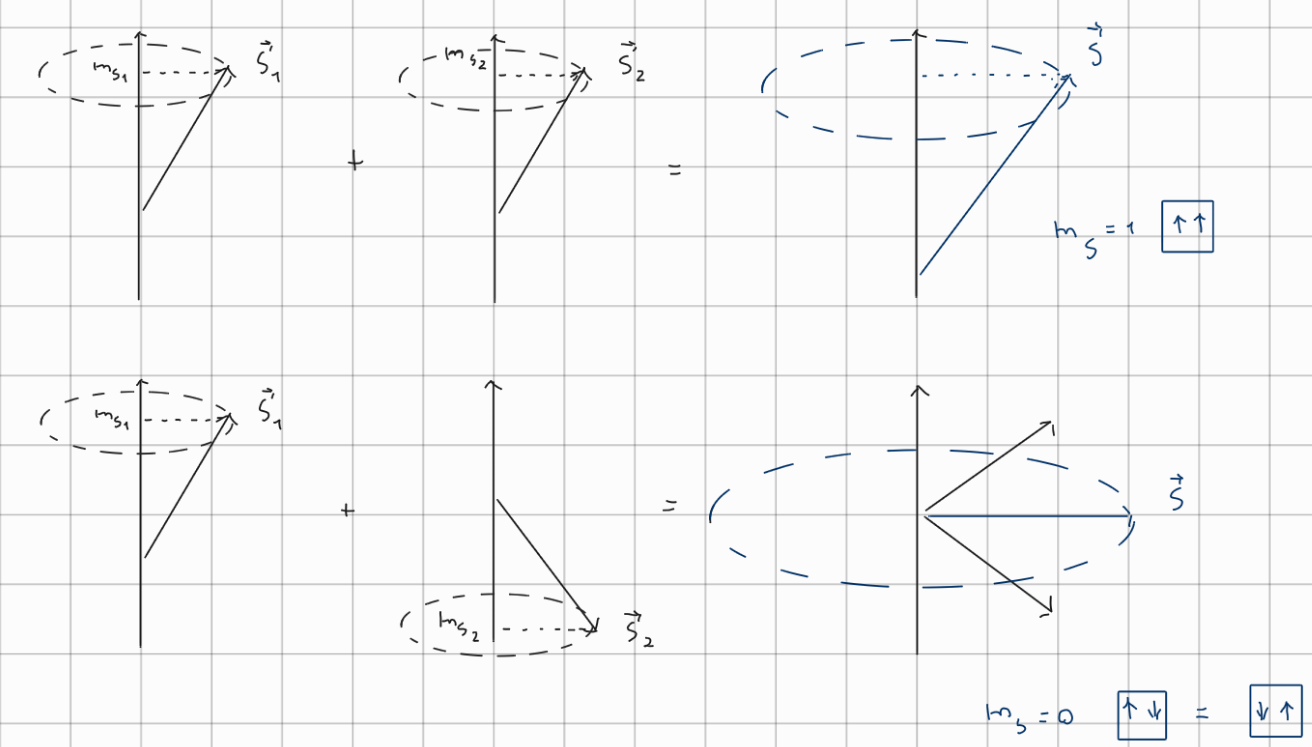
\includegraphics[width=0.8\linewidth]{immagini/2026-05-07-15-45-16.png}
    \end{figure}

\section{Momento Angolare Totale dell'Elettrone ($\vec{J}$)} %

Torniamo al singolo elettrone. Esso possiede contemporaneamente un momento orbitale $\vec{L}$ e uno spin intrinseco $\vec{S}$. Il suo \textbf{Momento Angolare Totale $\vec{J}$} è: %
\begin{equation}
    \vec{J} = \vec{L} + \vec{S} %
\end{equation}

Per il singolo elettrone, avendo sempre $s=1/2$, il numero quantico totale $j$ può valere: %
\begin{equation*}
    j = |l - s|, \dots, l + s \quad \Rightarrow \quad j = \left|l - \frac{1}{2}\right| \, , \, l + \frac{1}{2} %
\end{equation*}

Anche qui possiamo usare le due basi matematiche: %
\begin{itemize}
    \item[] \begin{figure}[H]
        \centering
        \begin{minipage}{0.3\textwidth}
            \centering
            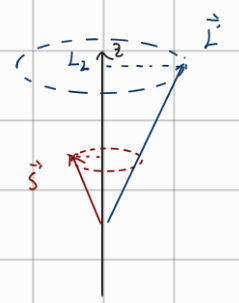
\includegraphics[width=0.8\linewidth]{immagini/2026-05-07-15-50-29.png}
        \end{minipage}\hfill
        \begin{minipage}{0.65\textwidth}
            $|l, m_l, s, m_s\rangle$ \textbf{(BASE DISACCOPPIATA):} Vede i due vettori $\vec{L}$ e $\vec{S}$ precessare indipendentemente attorno all'asse $z$. %
        \end{minipage}
    \end{figure}
    \item[] \begin{figure}[H]
        \centering
        \begin{minipage}{0.3\textwidth}
            \centering
            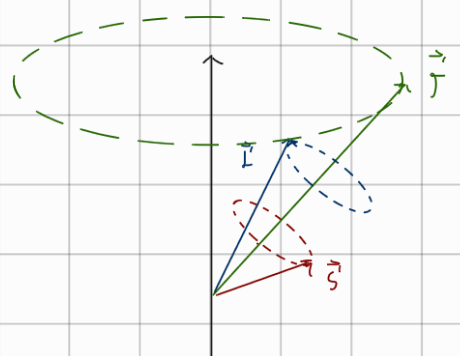
\includegraphics[width=\linewidth]{immagini/2026-05-07-15-50-57.png}
        \end{minipage}\hfill
        \begin{minipage}{0.65\textwidth}
            $|j, m_j, l, s\rangle$ \textbf{(BASE ACCOPPIATA):} $\vec{L}$ e $\vec{S}$ precessano accoppiati attorno al loro vettore somma $\vec{J}$, il quale a sua volta precessa rigidamente attorno all'asse $z$. %
            \textit{Da questo disegno si capisce perché $L_z$ e $S_z$ non sono rigorosamente costanti e non sono definiti in questa base (non compaiono i quanti $m_l$ e $m_s$): precessando attorno a $\vec{J}$, le loro singole proiezioni su $z$ oscillano nel tempo!} %
        \end{minipage}
    \end{figure}
\end{itemize}

\noindent
Qual è il momento magnetico totale $\vec{\mu}_j$ associato a questo elettrone che orbita e "spina" contemporaneamente? %
\begin{equation}
    \vec{\mu}_j = -g_j \mu_B \frac{\vec{J}}{\hbar} \qquad \text{e per la proiezione } z \text{:} \quad (\mu_j)_z = -g_j \mu_B m_j %
\end{equation}
Tuttavia, siccome il fattore giromagnetico orbitale ($g_l = 1$) è diverso da quello di spin ($g_s = 2$), la loro combinazione produce un fattore ibrido detto \textbf{Fattore di Landé} ($g_j$): %
\begin{equation}
    \boxed{ g_j = 1 + \frac{j(j+1) - l(l+1) + s(s+1)}{2j(j+1)} } %
\end{equation}

Applichiamo la teoria per prevedere i risultati sperimentali: %

\textbf{Esempio 1: Atomo di Idrogeno nello stato fondamentale (1s)} %
\begin{figure}[H]
    \centering
    \begin{minipage}{0.3\textwidth}
        \centering
        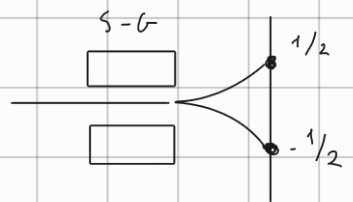
\includegraphics[width=\linewidth]{immagini/2026-05-07-15-54-54.png}
    \end{minipage}\hfill
    \begin{minipage}{0.65\textwidth}
        \begin{itemize}
            \item $l = 0$ (stato s), $s = 1/2$. %
            \item $j = |0 - 1/2| = 1/2$. %
            \item Essendo $l=0$, il momento magnetico è puramente di spin. La formula di Landé restituisce $g_j = g_s = 2$. %
            \item Valori di proiezione: $m_j = \pm 1/2$. %
            \item \textbf{Previsione:} In un campo di Stern-Gerlach, il fascio si dividerà in \textbf{2 macchie}. %
        \end{itemize}
    \end{minipage}
\end{figure}

\textbf{Esempio 2: Atomo di Idrogeno eccitato nello stato (2p)} %
\begin{figure}[H]
    \centering
    \begin{minipage}{0.3\textwidth}
        \centering
        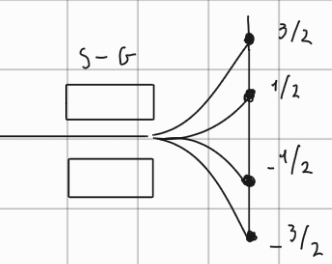
\includegraphics[width=\linewidth]{immagini/2026-05-07-15-55-06.png}
    \end{minipage}\hfill
    \begin{minipage}{0.65\textwidth}
        \begin{itemize}
            \item $l = 1$ (stato p), $s = 1/2$. %
            \item $j$ può valere $1 - 1/2 = 1/2$ oppure $1 + 1/2 = 3/2$. %
            \item Prendiamo lo stato con $j = 3/2$. Le proiezioni ammesse sono $m_j = -3/2, -1/2, 1/2, 3/2$. %
            \item \textbf{Previsione:} Il fascio si dividerà in \textbf{4 macchie} distinte! %
        \end{itemize}
    \end{minipage}
\end{figure}

\noindent
L'esperimento conferma puntualmente la teoria. L'integrazione di Spin e momento Orbitale funziona in modo perfetto. %

\section{Effetto Einstein-de Haas} %

Una dimostrazione macroscopica del legame tra momento magnetico e momento angolare è l'esperimento di Einstein-de Haas. Consideriamo un cilindro di materiale ferromagnetico sospeso a un filo. %
Sia $\vec{M} = n \vec{\mu}$ la densità di dipolo magnetico. Sappiamo che nei ferromagneti il momento orbitale medio è nullo (Quenching: $\langle \vec{L} \rangle = 0$), quindi la magnetizzazione è dovuta solo allo \textbf{Spin}: %
\begin{equation*}
    \vec{M} = n \vec{\mu}_s \quad \Rightarrow \quad (\mu_s)_z = -g_s \mu_B m_s \quad \Rightarrow \quad M = -n g_s \mu_B m_s %
\end{equation*}
\begin{figure}[H]
    \centering
    \begin{minipage}{0.2\textwidth}
        \centering
        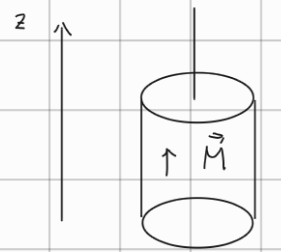
\includegraphics[width=\linewidth]{immagini/2026-05-07-15-56-29.png}
    \end{minipage}\hfill
    \begin{minipage}{0.75\textwidth}
        Se il cilindro è magnetizzato verso l'alto ($\vec{M} \uparrow$), poiché $\vec{\mu}_s$ ha verso opposto allo spin (carica negativa dell'elettrone), gli spin saranno orientati verso il basso: $S_z = -\hbar/2$. %
    \end{minipage}
\end{figure}

\begin{figure}[H]
    \centering
    \begin{minipage}{0.2\textwidth}
        \centering
        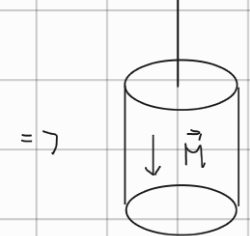
\includegraphics[width=\linewidth]{immagini/2026-05-07-15-56-42.png}
    \end{minipage}\hfill
    \begin{minipage}{0.75\textwidth}
        Se ora \textbf{inverto il campo magnetico} esterno, la magnetizzazione si inverte ($\vec{M} \downarrow$), costringendo gli spin a ribaltarsi verso l'alto ($S_z = +\hbar/2$). La variazione di magnetizzazione è associata a una variazione del momento angolare di spin: %
    \end{minipage}
\end{figure}
\begin{equation*}
    \Delta M = n g_s \mu_B \frac{\Delta S_z}{\hbar} = n g_s \mu_B \Delta m_s %
\end{equation*}

\noindent
Poiché il cilindro è un sistema isolato, \textbf{il Momento Angolare Totale si deve conservare}! %
\begin{equation*}
    \Delta J_z = \Delta L_z + \Delta S_z = 0 \quad \Rightarrow \quad \Delta L_z = -\Delta S_z = -\frac{\hbar \Delta M}{n g_s \mu_B} \hat{n}_z %
\end{equation*}
Per compensare il ribaltamento microscopico degli spin, il cilindro intero (macroscopico) acquisisce un momento angolare orbitale $\Delta L_z$ e \textbf{inizia a ruotare} meccanicamente sul proprio asse con velocità $\omega = L_z / I$! %

\section{Interazione Spin-Orbita} %

Finora abbiamo considerato $\vec{S}$ e $\vec{L}$ come indipendenti. In realtà, essi interagiscono. %
Mettiamoci nel \textbf{Sistema di Riferimento dell'elettrone} ($e^-$ in quiete). Da questa prospettiva, è il nucleo (carica $+Ze$) a ruotargli attorno a distanza $r$ con velocità $v$. %
Questo moto nucleare costituisce una spira di corrente $i = \frac{Ze}{T} = \frac{Z e v}{2\pi r}$, che genera un campo magnetico $\vec{B}$ al centro (dove sta l'elettrone): %
\begin{figure}[H]
    \centering
    \begin{minipage}{0.3\textwidth}
        \centering
        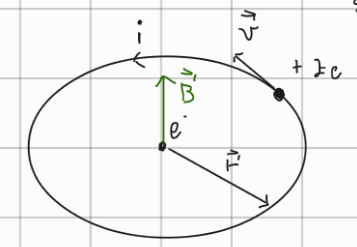
\includegraphics[width=\linewidth]{immagini/2026-05-07-15-59-02.png}
    \end{minipage}\hfill
    \begin{minipage}{0.65\textwidth}
        \begin{equation*}
            |\vec{B}| = \frac{\mu_0 i}{2r} = \frac{\mu_0 Z e v}{4\pi r^2} %
        \end{equation*}
        Moltiplichiamo numeratore e denominatore per la massa $m$ dell'elettrone, per far apparire il momento orbitale $L = mvr$. Usiamo inoltre la relazione di Maxwell $1/c^2 = \varepsilon_0 \mu_0$: %
        \begin{equation*}
            |\vec{B}| = \frac{\mu_0 Z e}{4\pi m r^3} (mvr) = \frac{\mu_0 \varepsilon_0 Z e}{4\pi \varepsilon_0 m r^3} |\vec{L}| \quad \Rightarrow \quad \vec{B} = \frac{Ze}{4\pi\varepsilon_0 m c^2 r^3} \vec{L} %
        \end{equation*}
    \end{minipage}
\end{figure}

\begin{figure}[H]
    \centering
    \begin{minipage}{0.3\textwidth}
        \centering
        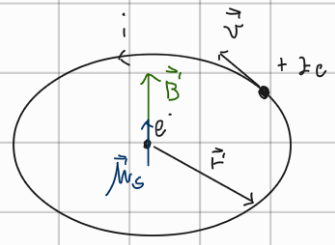
\includegraphics[width=\linewidth]{immagini/2026-05-07-16-00-07.png}
    \end{minipage}\hfill
    \begin{minipage}{0.65\textwidth}
        L'elettrone possiede un momento magnetico di spin $\vec{\mu}_s$. Trovandosi immerso nel campo $\vec{B}$ generato dalla sua stessa orbita, subirà un'energia potenziale di interazione: %
        \begin{equation*}
            U = -\vec{\mu}_s \cdot \vec{B} \quad \text{(Accoppia lo Spin e le Orbite!)} %
        \end{equation*}
    \end{minipage}
\end{figure}

\noindent
\textbf{Precessione di Thomas:} Il calcolo appena fatto vale nel sistema solidale all'elettrone accelerato. Per tornare al sistema di riferimento del \textit{laboratorio} (protone in quiete), è necessario applicare le trasformazioni di Lorentz della Relatività. I calcoli (complessi) mostrano che emerge un fattore cinematico correttivo esattamente pari a $\frac{1}{2}$: %
\begin{figure}[H]
    \centering
    \begin{minipage}{0.3\textwidth}
        \centering
        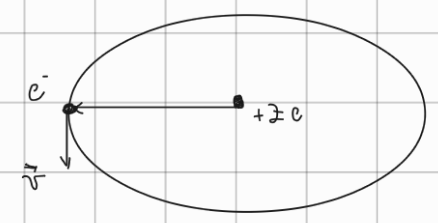
\includegraphics[width=\linewidth]{immagini/2026-05-07-16-01-06.png}
    \end{minipage}\hfill
    \begin{minipage}{0.65\textwidth}
        \begin{equation*}
            \Delta E_{SO} = -\frac{1}{2} \vec{\mu}_s \cdot \vec{B} %
        \end{equation*}
        Sostituendo $\vec{\mu}_s = -g_s \mu_B \frac{\vec{S}}{\hbar}$ (con $g_s = 2$) e l'espressione di $\vec{B}$: %
        \begin{align*}
            \Delta E_{SO} = \frac{1}{2} \left( 2 \frac{e\hbar}{2m} \right) \frac{\vec{S}}{\hbar} \cdot \left( \frac{Ze}{4\pi\varepsilon_0 m c^2 r^3} \vec{L} \right) \quad \Rightarrow \\
            \quad \boxed{ \Delta E_{SO} = \frac{Z e^2}{8\pi\varepsilon_0 m^2 c^2 r^3} \vec{S} \cdot \vec{L} } %
        \end{align*}
    \end{minipage}
\end{figure}

\noindent
Valutiamo quanto è "forte" questa correzione rispetto all'energia imperturbata di Bohr. Approssimando $S \sim L \sim \hbar$, $r \sim a_0 = \frac{4\pi\varepsilon_0\hbar^2}{me^2}$, ed $E \sim Ry = \frac{me^4}{2(4\pi\varepsilon_0\hbar)^2}$: %
\begin{equation*}
    \Delta E_{SO} \simeq \frac{Z e^2}{8\pi\varepsilon_0 m^2 c^2} \left( \frac{me^2}{4\pi\varepsilon_0\hbar^2} \right)^3 \cdot \hbar^2 = \dots = Z \left[ \frac{me^4}{2(4\pi\varepsilon_0\hbar)^2} \right] \left[ \frac{e^2}{4\pi\varepsilon_0 c\hbar} \right]^2 = Z \cdot Ry \cdot \alpha^2 %
\end{equation*}

Dove abbiamo isolato la fondamentale \textbf{Costante di Struttura Fine ($\alpha$)}: %
\begin{equation}
    \alpha \equiv \frac{e^2}{4\pi\varepsilon_0 c\hbar} \simeq \frac{1}{137} %
\end{equation}
La correzione relativa è quindi \boxed{\frac{\Delta E}{E} \approx \alpha^2 \approx 10^{-4}}. È una variazione piccola, ma non trascurabile! %

\noindent
Possiamo generalizzare l'espressione dell'energia di Spin-Orbita per un qualunque potenziale centrale $V(r)$. Isoliamo la forza elettrostatica all'interno dell'espressione, sapendo che essa è pari alla derivata del potenziale: %
\begin{equation*}
    F_{el} = -|\nabla V| = \frac{dV}{dr} %
\end{equation*}

\begin{equation}
    \Delta E_{SO} = \frac{1}{2m^2c^2} \underbrace{ \frac{Z e^2}{4\pi\varepsilon_0 r^2} }_{F_{el}} \frac{1}{r} \vec{S} \cdot \vec{L} \quad \Rightarrow \quad \boxed{ \Delta E_{SO} = \frac{1}{2m^2c^2} \left( \frac{1}{r} \frac{dV}{dr} \right) \vec{S} \cdot \vec{L} } %
\end{equation}

\noindent
Definiamo quindi il rispettivo operatore Hamiltoniano di Spin-Orbita $\hat{H}_{SO}$. L'Hamiltoniana completa $\hat{H}$ per l'atomo reale diventa la somma dell'energia cinetica (Laplaciano $\Delta$), dell'energia potenziale centrale e della nuova perturbazione: %
\begin{equation}
    \hat{H}_{SO} = \frac{Z e^2}{8\pi\varepsilon_0 m^2 c^2 r^3} \hat{\vec{S}} \cdot \hat{\vec{L}} \quad \Rightarrow \quad \boxed{ \hat{H} = -\frac{\hbar^2}{2m}\Delta + \hat{V}(r) + \hat{H}_{SO} } %
\end{equation}

\begin{quote}
    \textbf{Nota Matematica:} Con l'aggiunta del termine misto $\hat{\vec{S}} \cdot \hat{\vec{L}}$, \textbf{NON C'È PIÙ UNA SOLUZIONE ANALITICA DIRETTA} all'equazione differenziale. % \\
    Lo si risolve con la \textbf{Teoria delle Perturbazioni NON dipendente dal tempo} (utilizzando, come visto in precedenza, la Base Accoppiata $|j, m_j, l, s\rangle$). %
\end{quote}

\subsection{Sdoppiamento dei Livelli (Doppietti)} %

Dobbiamo risolvere il sistema con la teoria delle perturbazioni \textbf{UTILIZZANDO LA BASE ACCOPPIATA} $|j, m_j, l, s\rangle$, poiché in questa base $\hat{\vec{S}} \cdot \hat{\vec{L}} = \frac{1}{2}(\hat{J}^2 - \hat{L}^2 - \hat{S}^2)$ è perfettamente diagonale! %

\noindent
Fisicamente, l'interazione Spin-Orbita spezza la degenerazione dei livelli energetici $l$ in due sottolivelli (\textbf{Doppietti di Spin-Orbita}): %
\begin{figure}[H]
    \centering
    \begin{minipage}{0.35\textwidth}
        \centering
        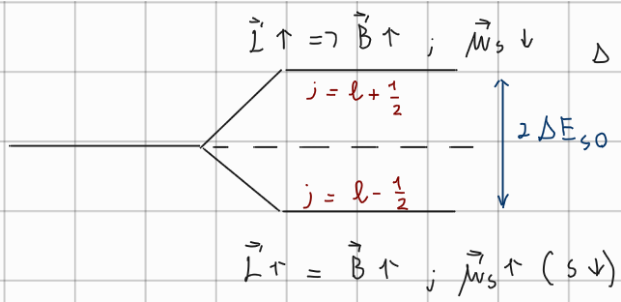
\includegraphics[width=\linewidth]{immagini/2026-05-07-17-22-12.png}
    \end{minipage}\hfill
    \begin{minipage}{0.65\textwidth}
        \begin{itemize}
            \item Se $\vec{L}$ e $\vec{S}$ sono \textit{concordi} ($\vec{L} \uparrow \Rightarrow \vec{B} \uparrow$, ma $\vec{\mu}_s \downarrow$). L'energia di interazione $\Delta E_{SO} = -\vec{\mu}_s \cdot \vec{B}$ è \textbf{POSITIVA}. Il livello energetico subisce un aumento. Si tratta dello stato con $j = l + 1/2$. %
            \item Se $\vec{L}$ e $\vec{S}$ sono \textit{discordi} ($\vec{L} \uparrow \Rightarrow \vec{B} \uparrow$, ma $\vec{\mu}_s \uparrow$). L'energia di interazione è \textbf{NEGATIVA}. Il livello energetico si abbassa. Si tratta dello stato con $j = l - 1/2$. %
        \end{itemize}
    \end{minipage}
\end{figure}

\noindent
Questo "splitting" spiega esattamente perché negli spettri atomici (come le famose righe del Sodio) molte singole linee di emissione, se guardate ad altissima risoluzione, si rivelano essere in realtà due linee vicinissime! %

\end{document}